\section{Extrinsic calibration}

\begin{figure}
  \centering
  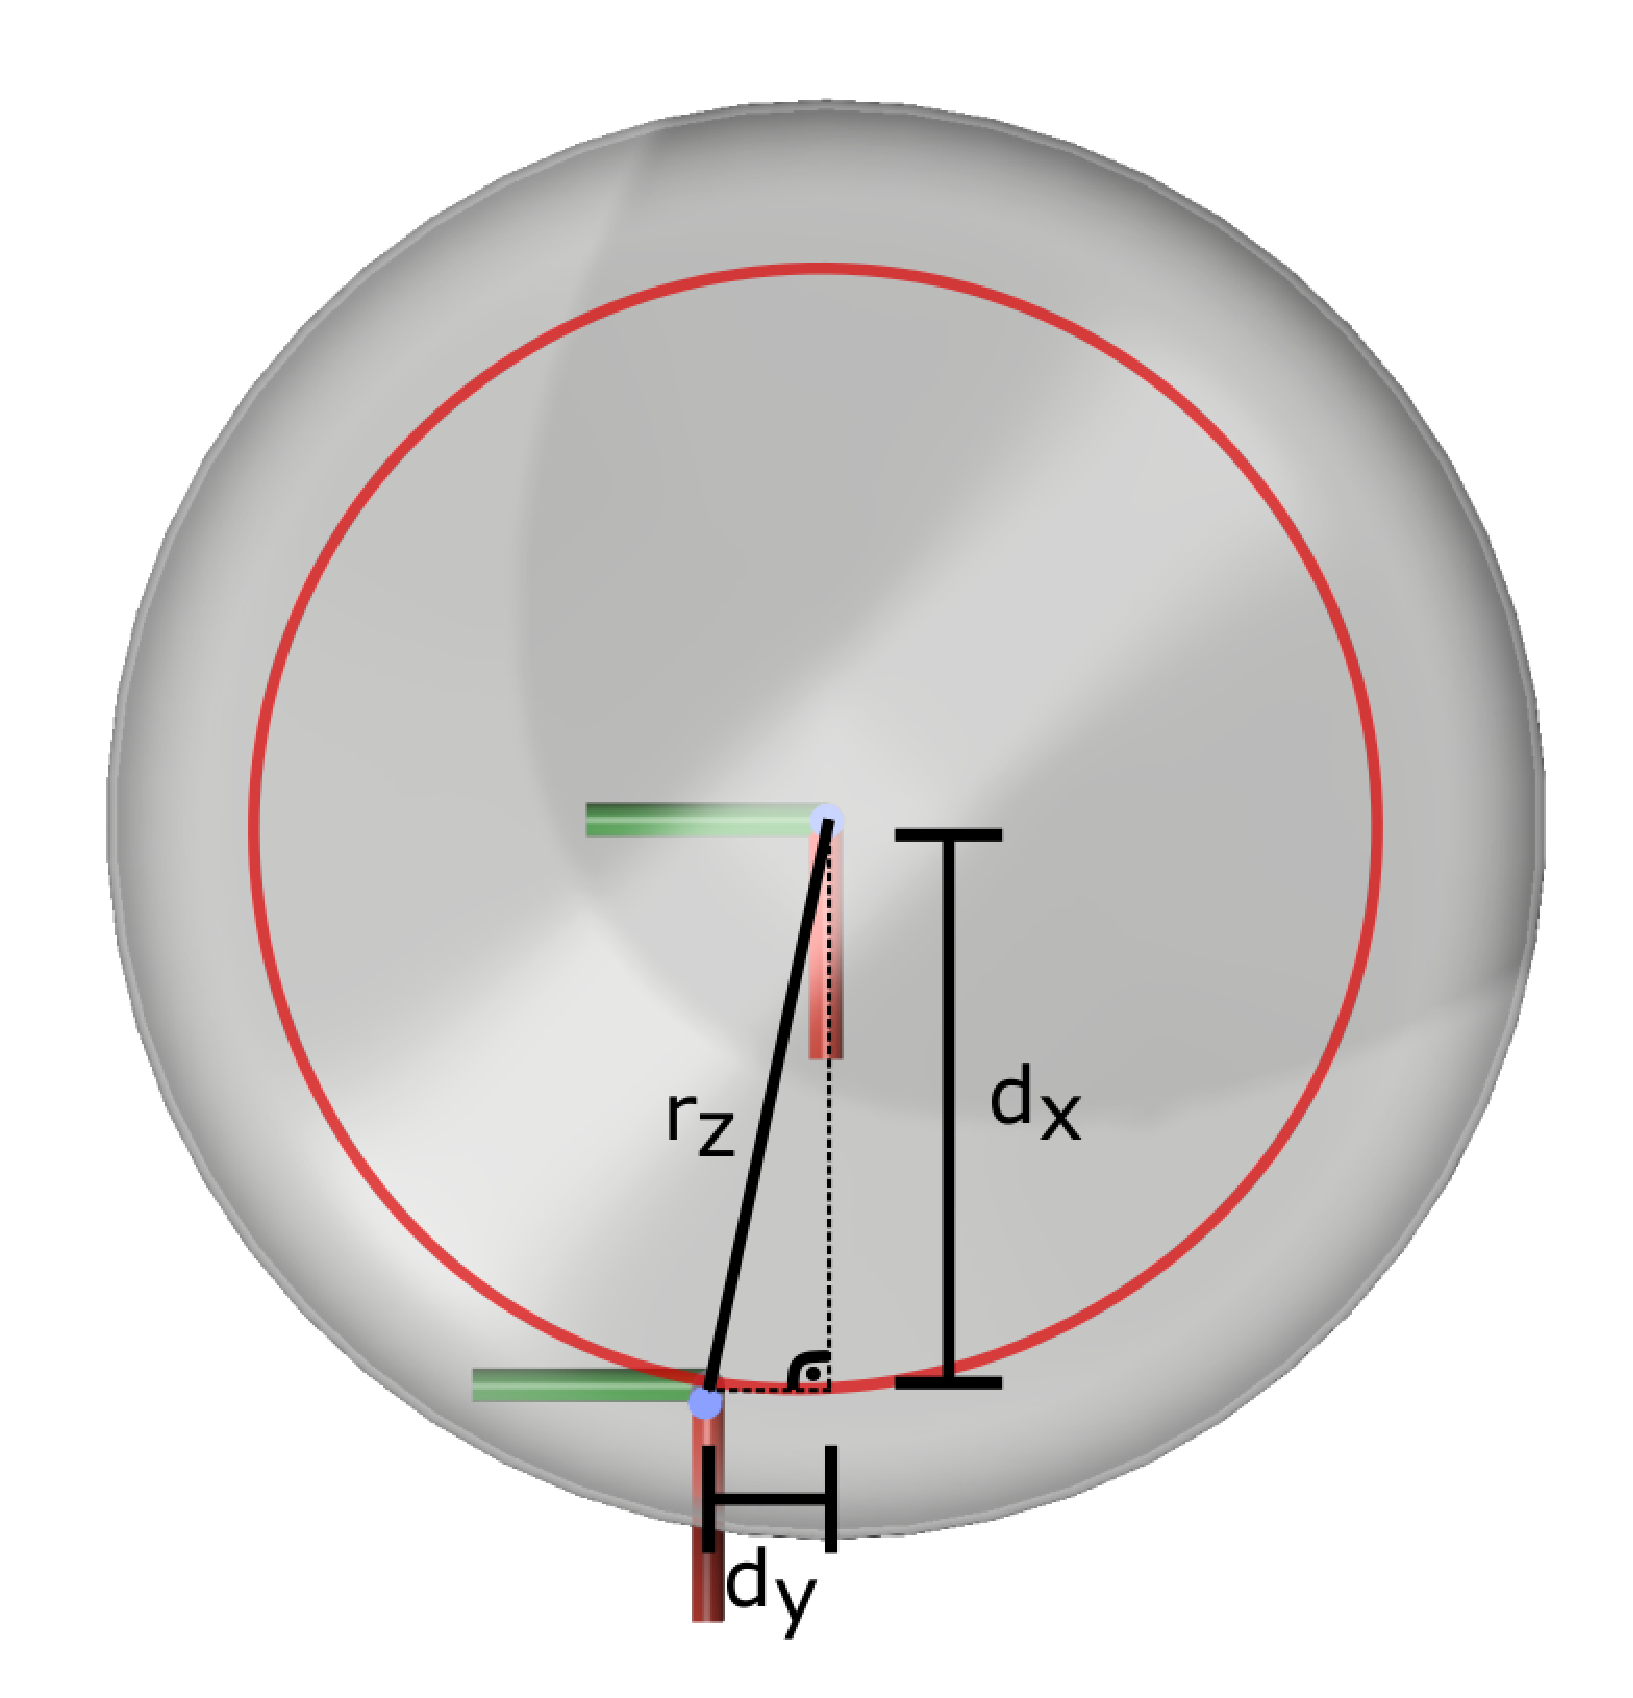
\includegraphics[width=.5\linewidth]{img/calibsphere}
  \caption{Calibration principle of a sensor inside a ball, illustrated in one axis.}
  \label{fig:calibsphere}
\end{figure}

\begin{figure}
  \centering
  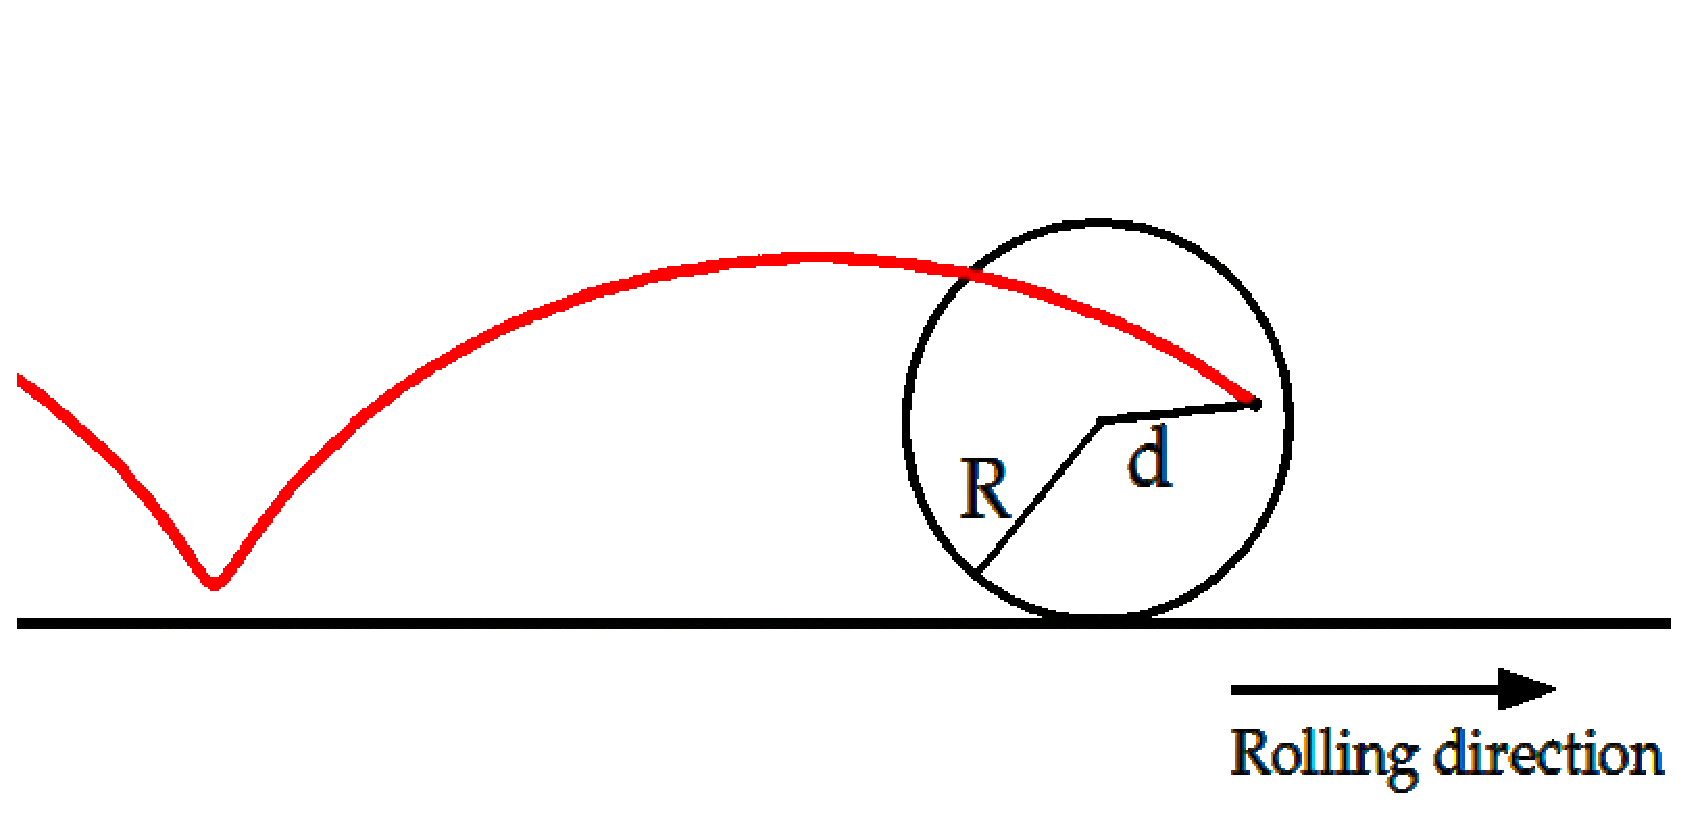
\includegraphics[width=\linewidth]{img/trochoidanim}
  \caption{Trochoid anim.}
  \label{fig:trochoidanim}
\end{figure}

\begin{figure*}
  \centering
  \includegraphics[width=\linewidth]{img/srr_trochoid}
  \caption{Ground turth image.}
  \label{fig:srrtrochoid}
\end{figure*}

\begin{figure}
  \centering
  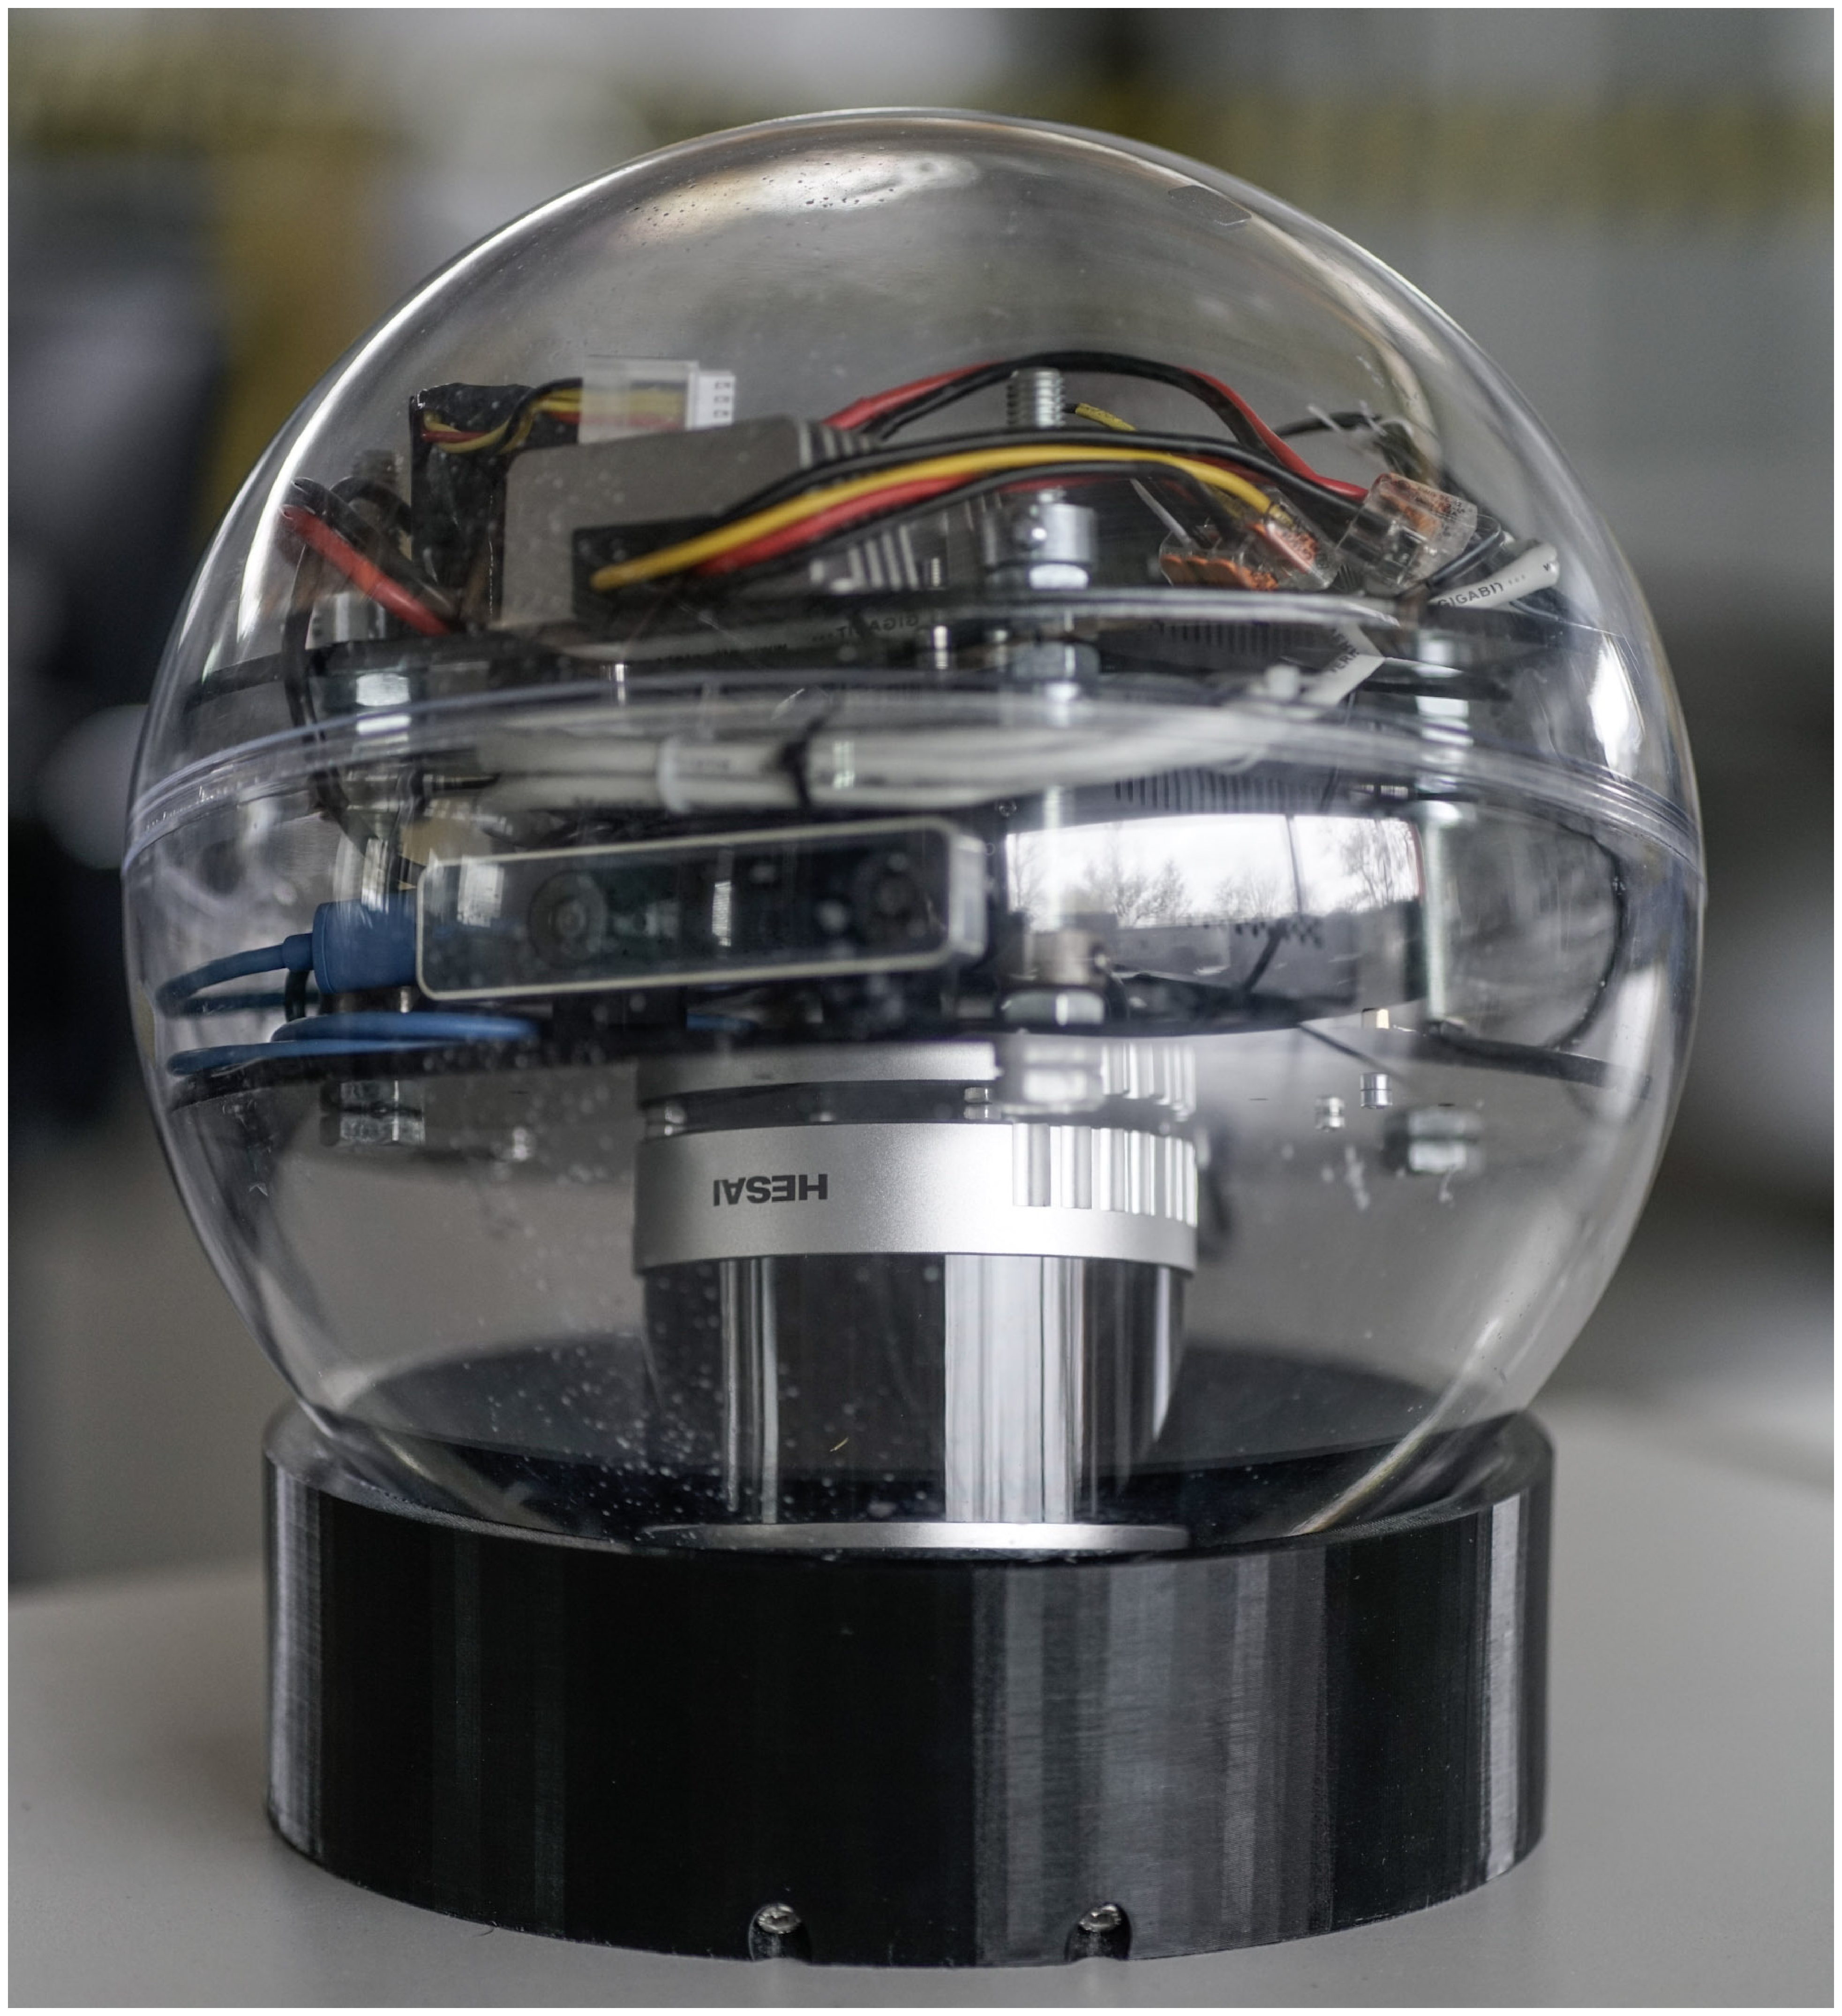
\includegraphics[height=.17\textheight]{img/sphere_calib}
  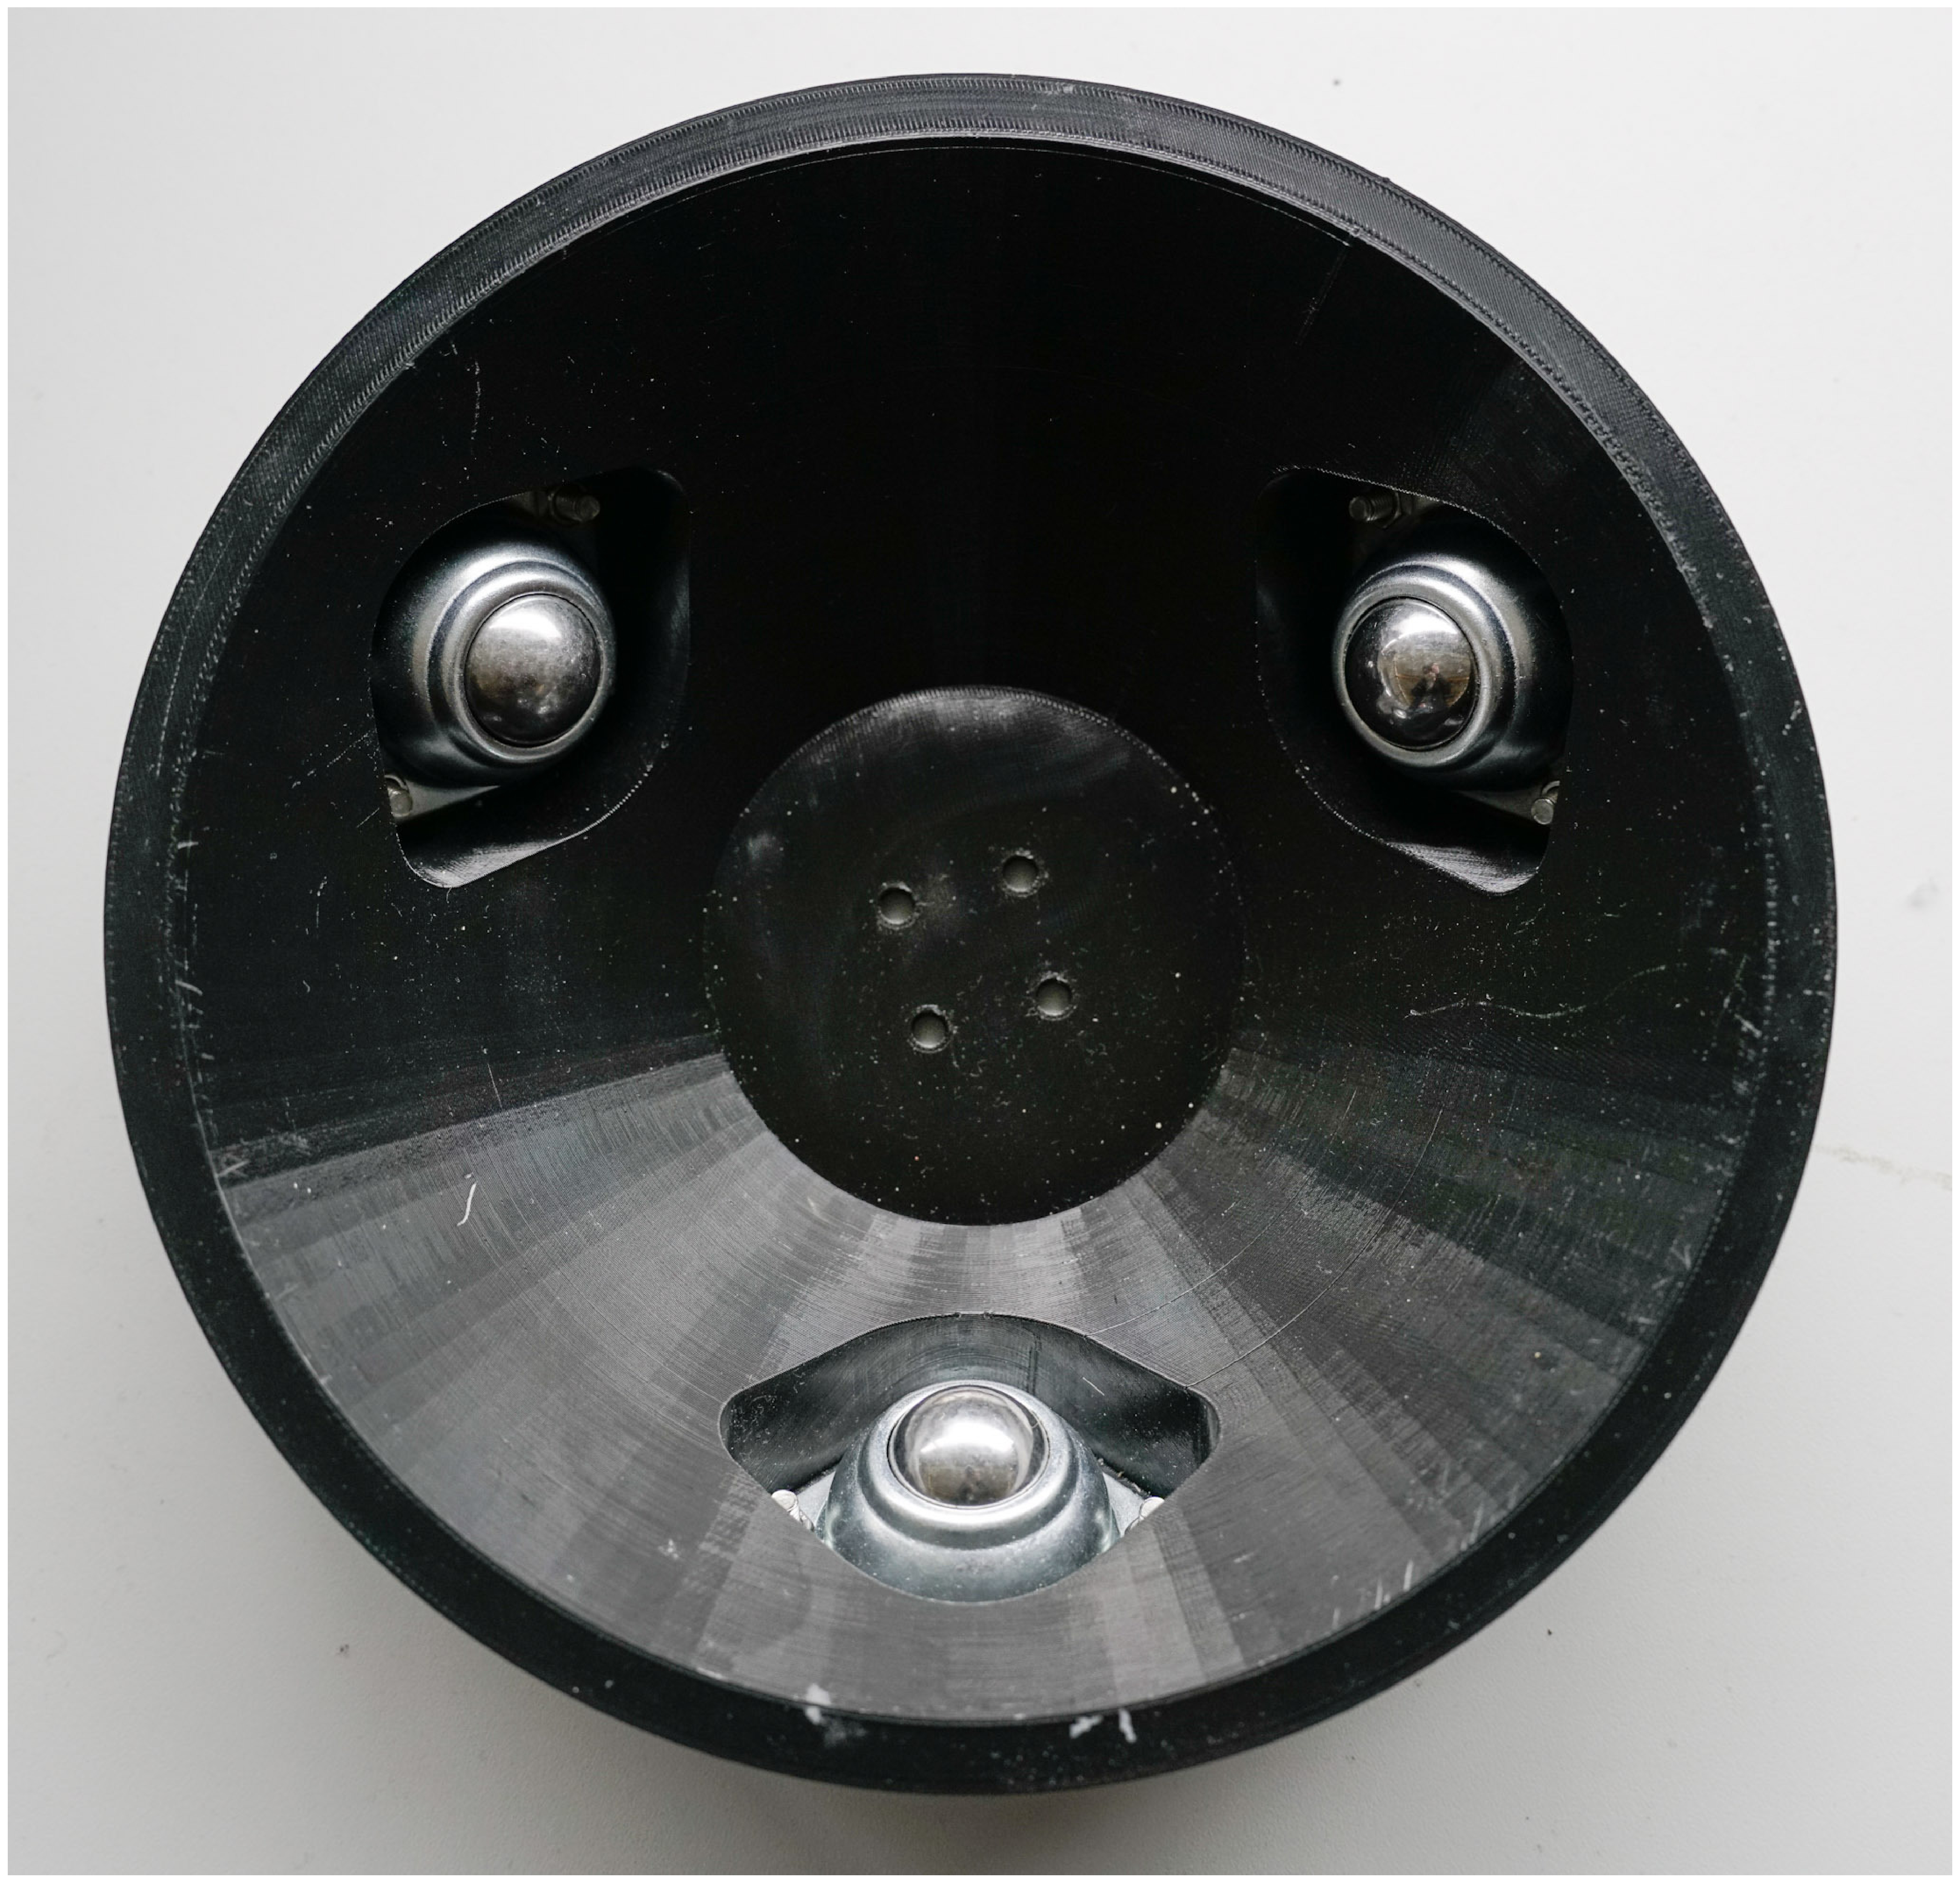
\includegraphics[height=.17\textheight]{img/calib_station}
  \caption{Calib station.}
  \label{fig:calibstation}
\end{figure}

\begin{figure}
  \centering
  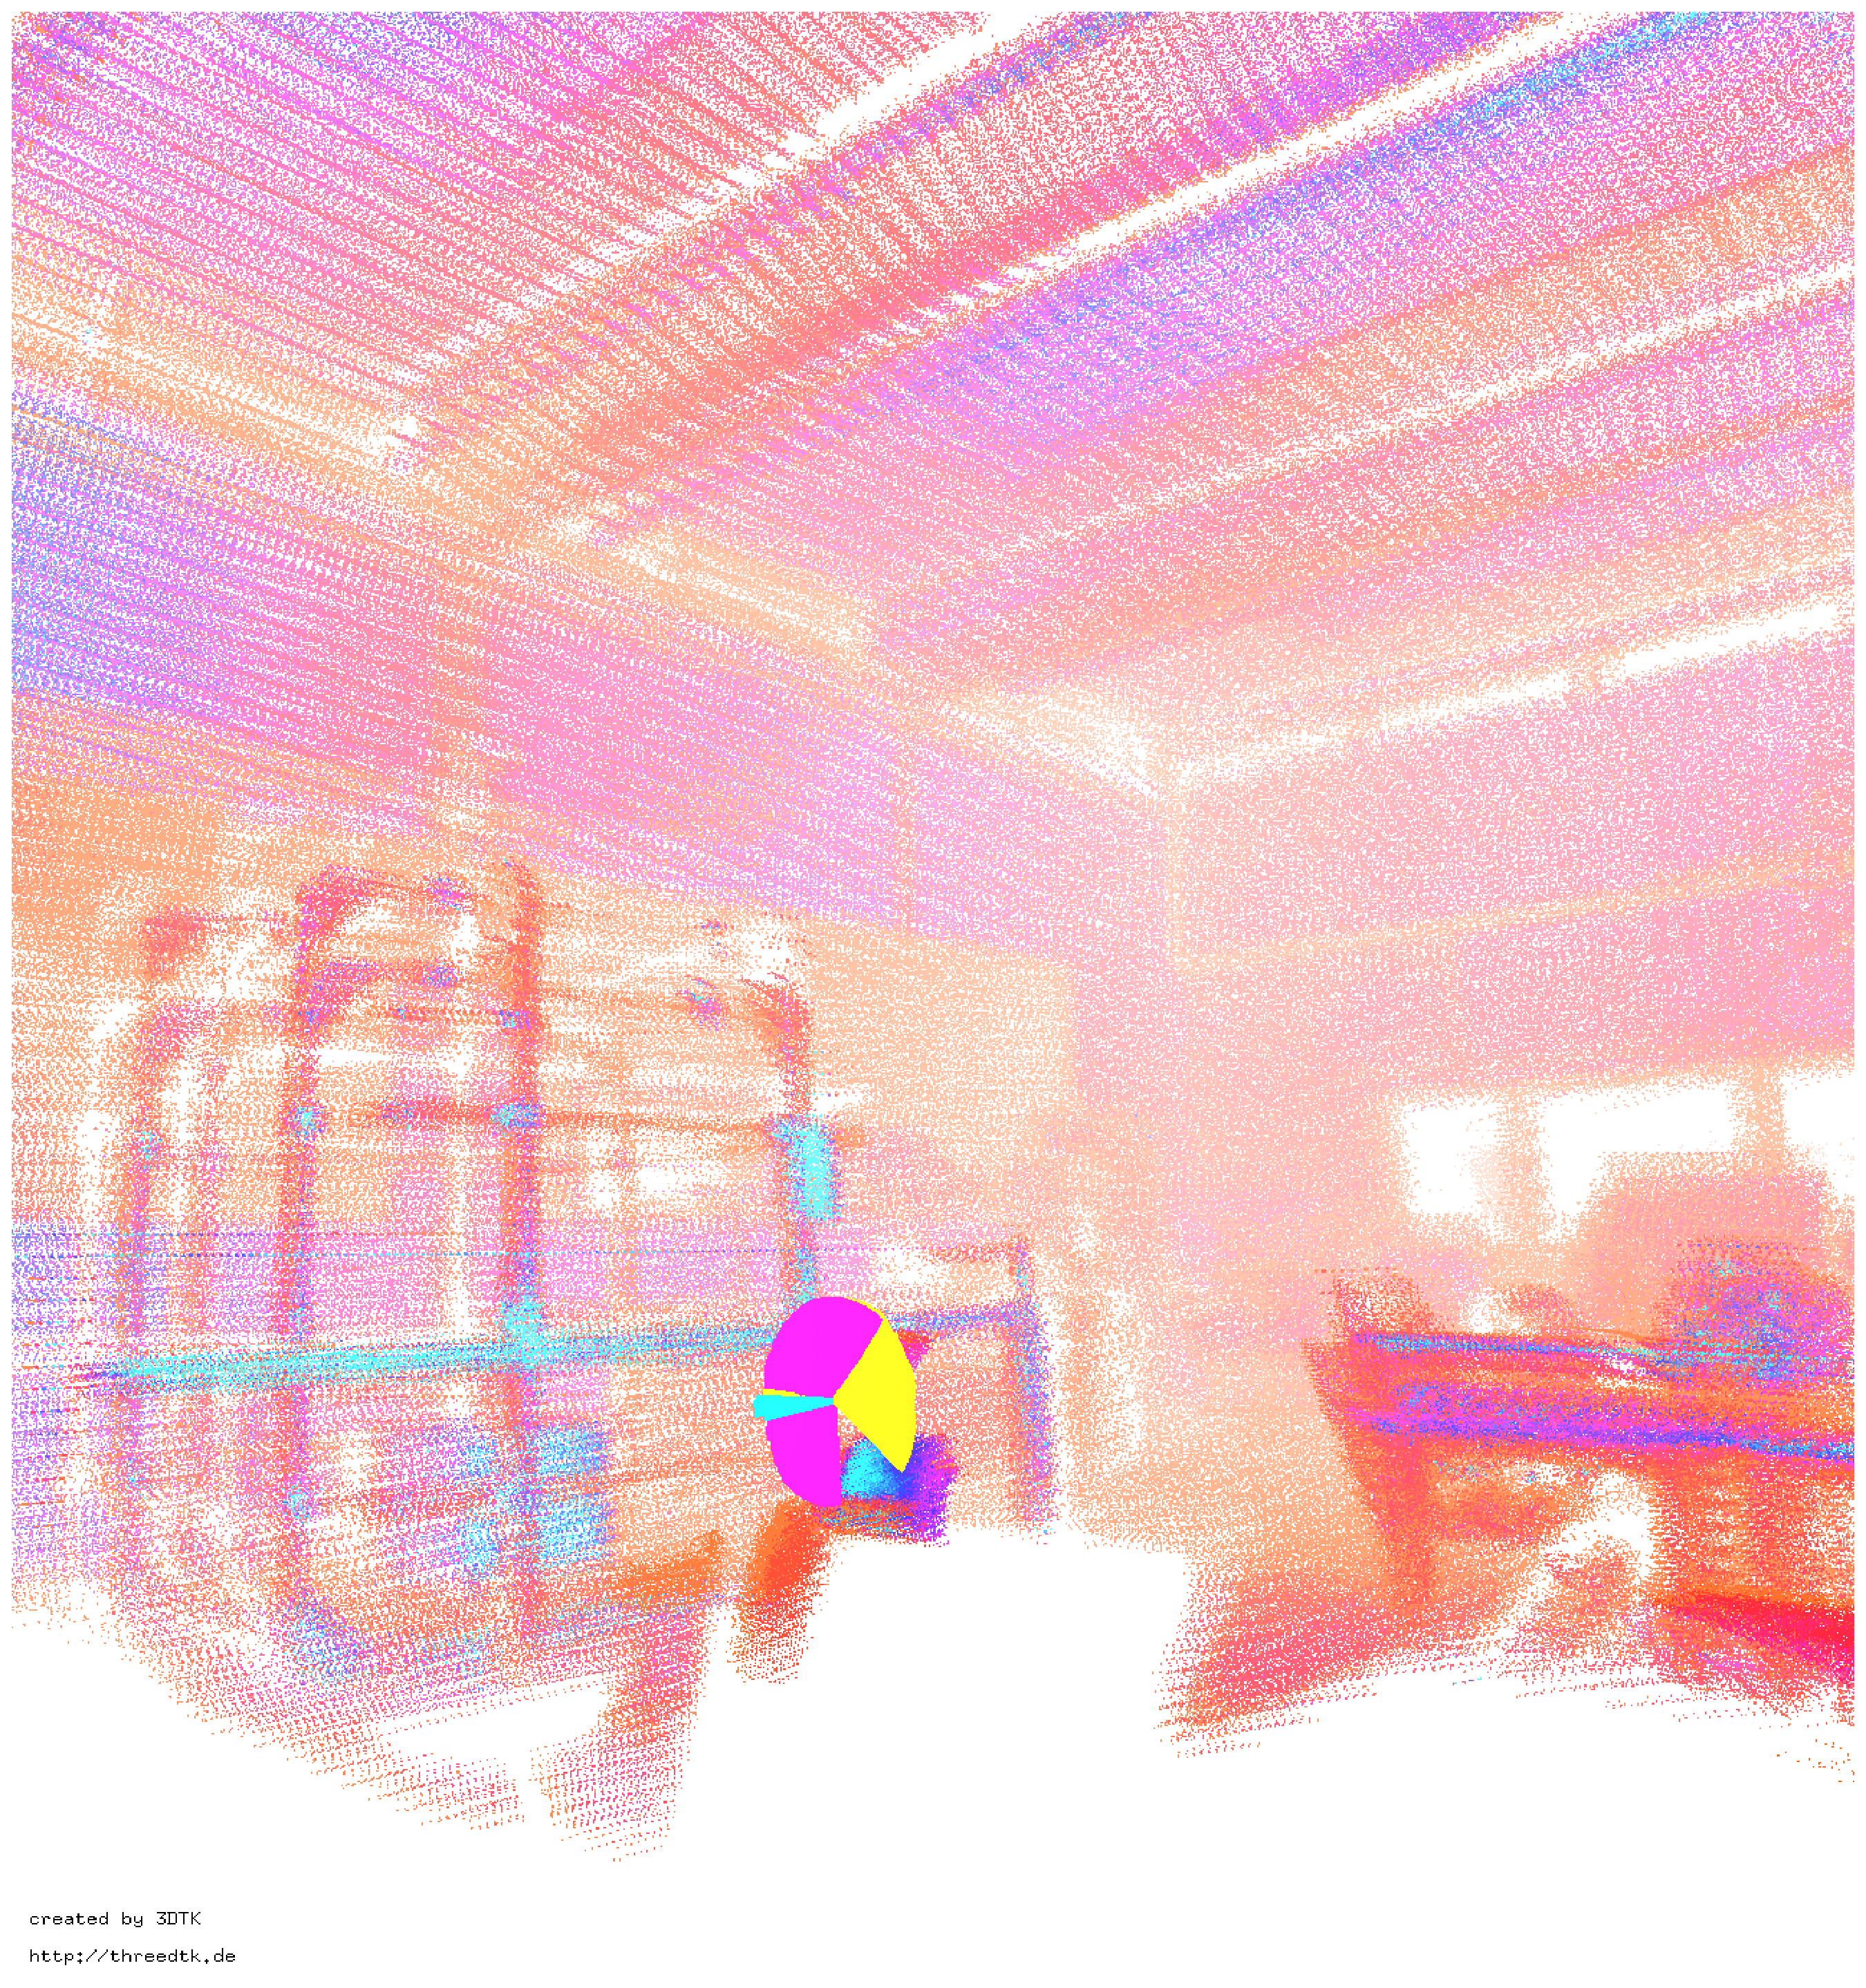
\includegraphics[width=.32\linewidth]{img/cam_rolls_before}
  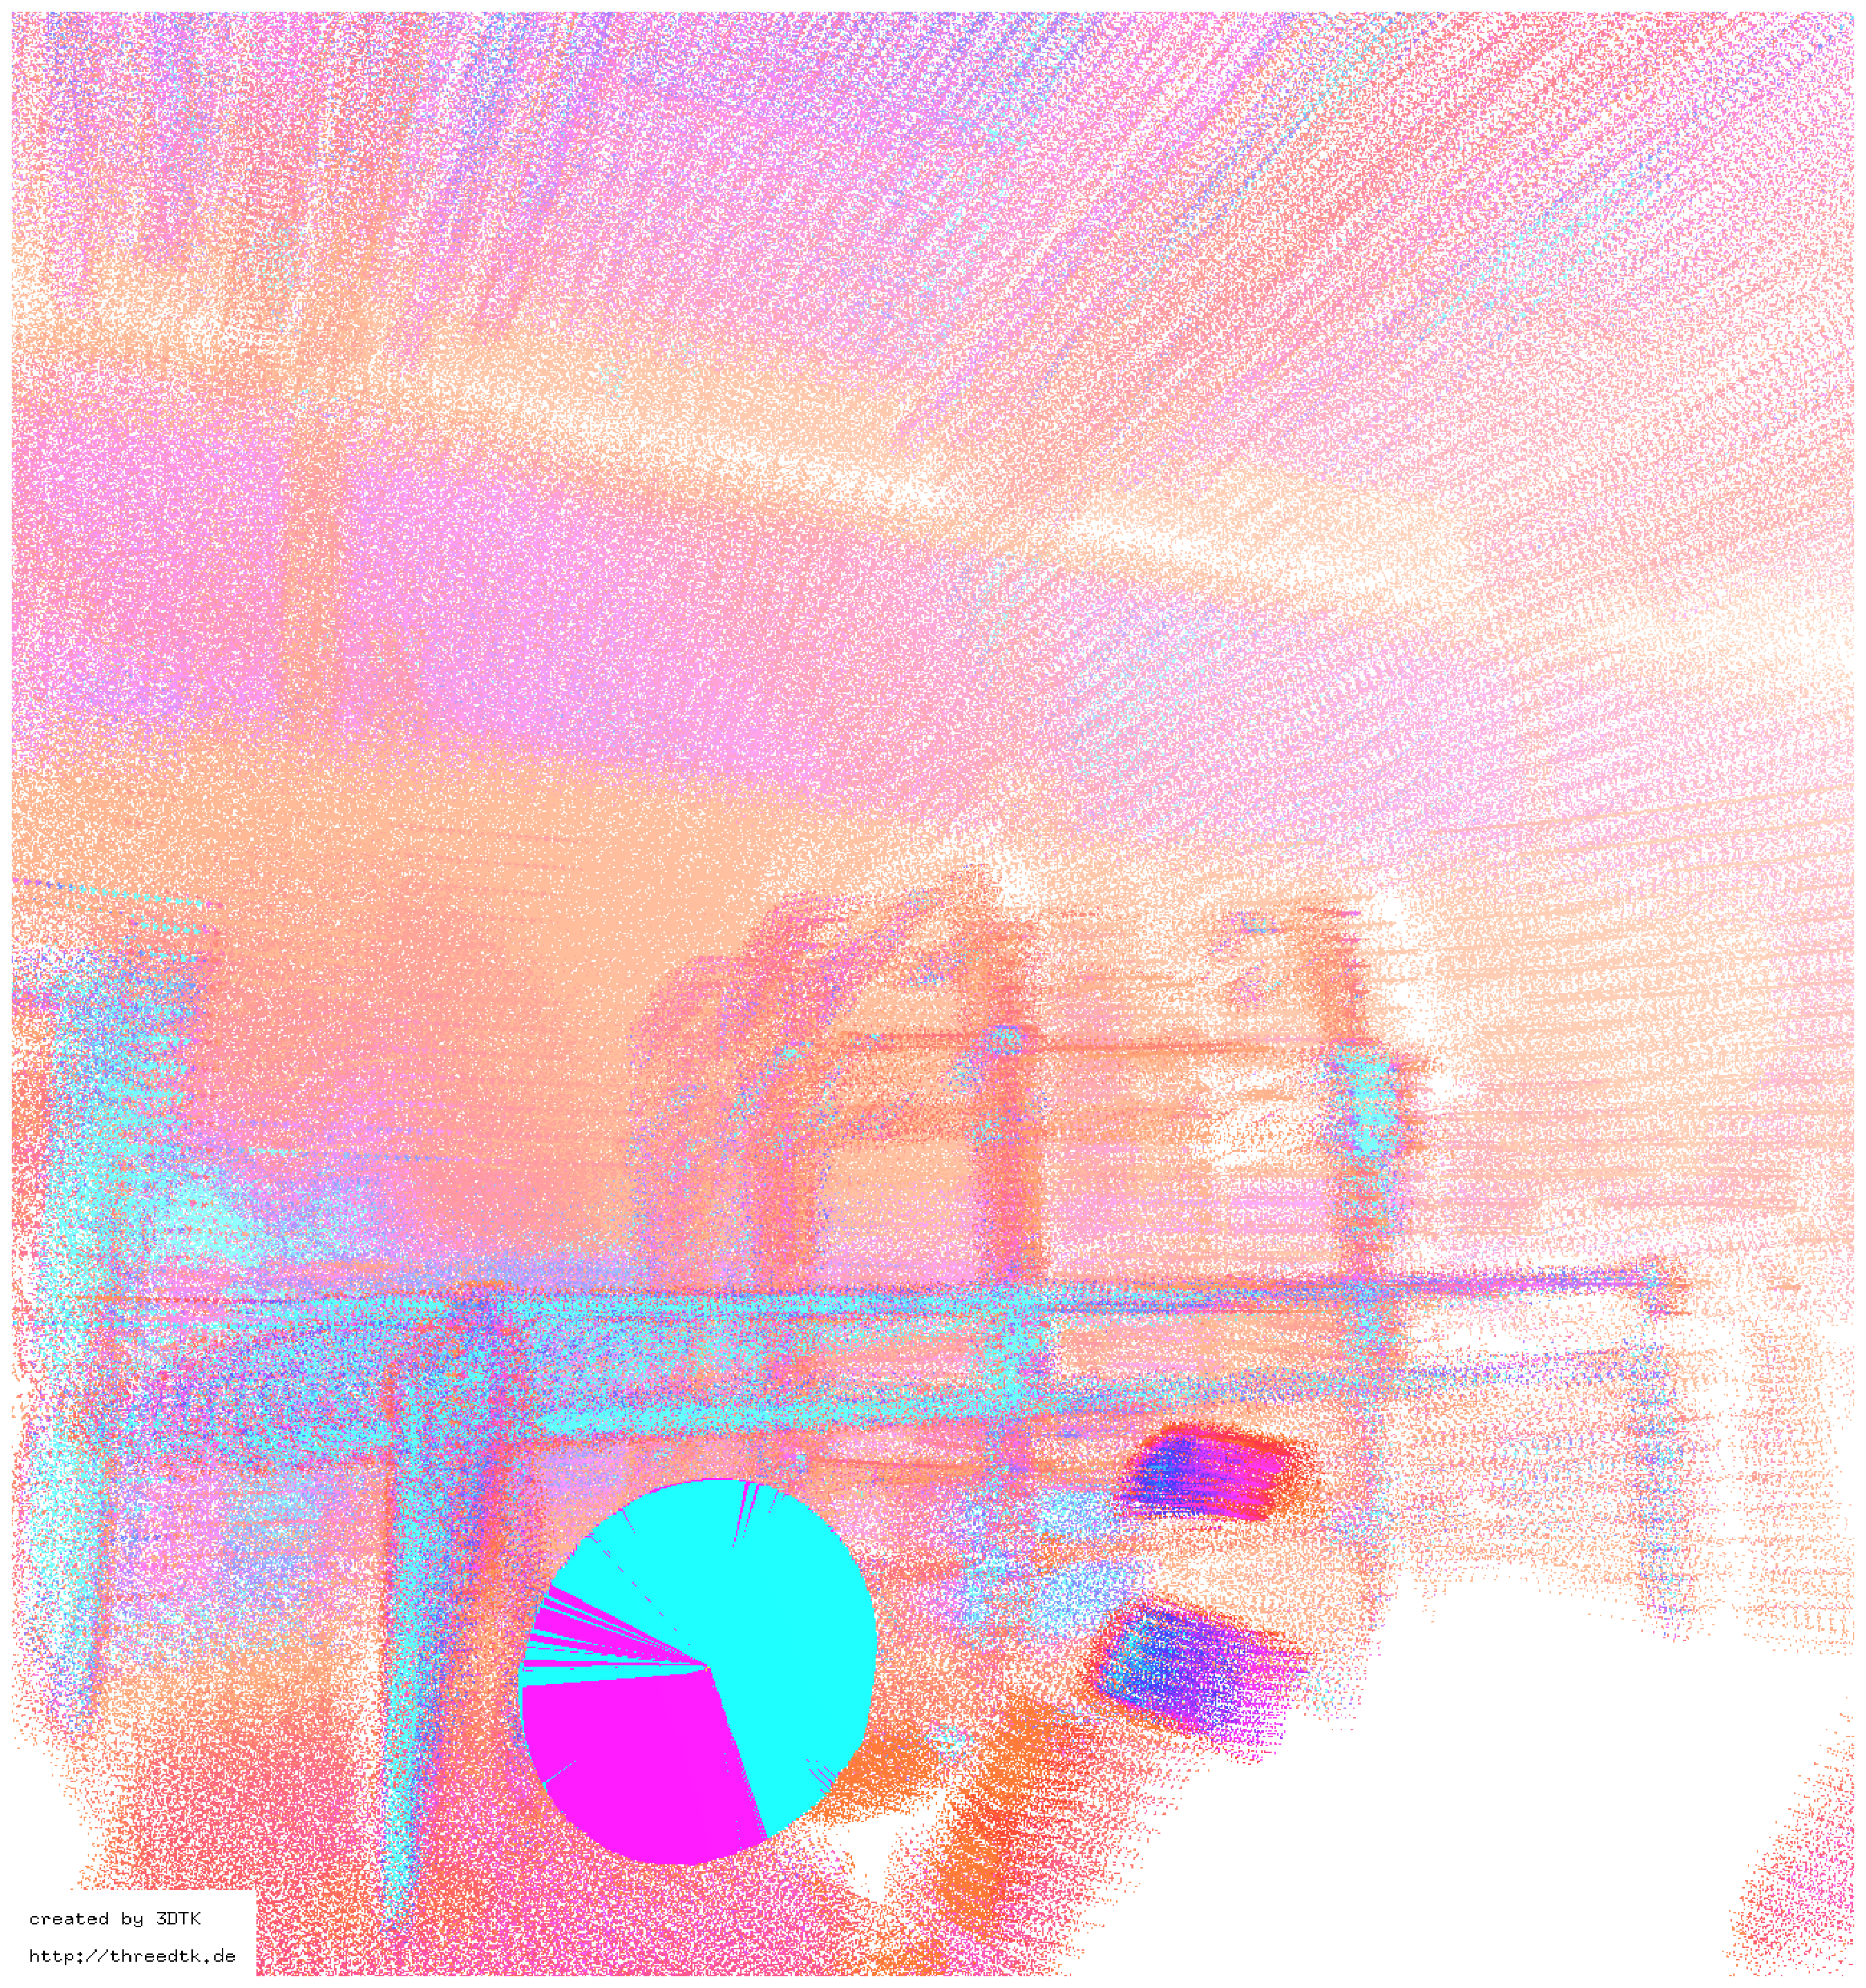
\includegraphics[width=.32\linewidth]{img/cam_pitches_before}
  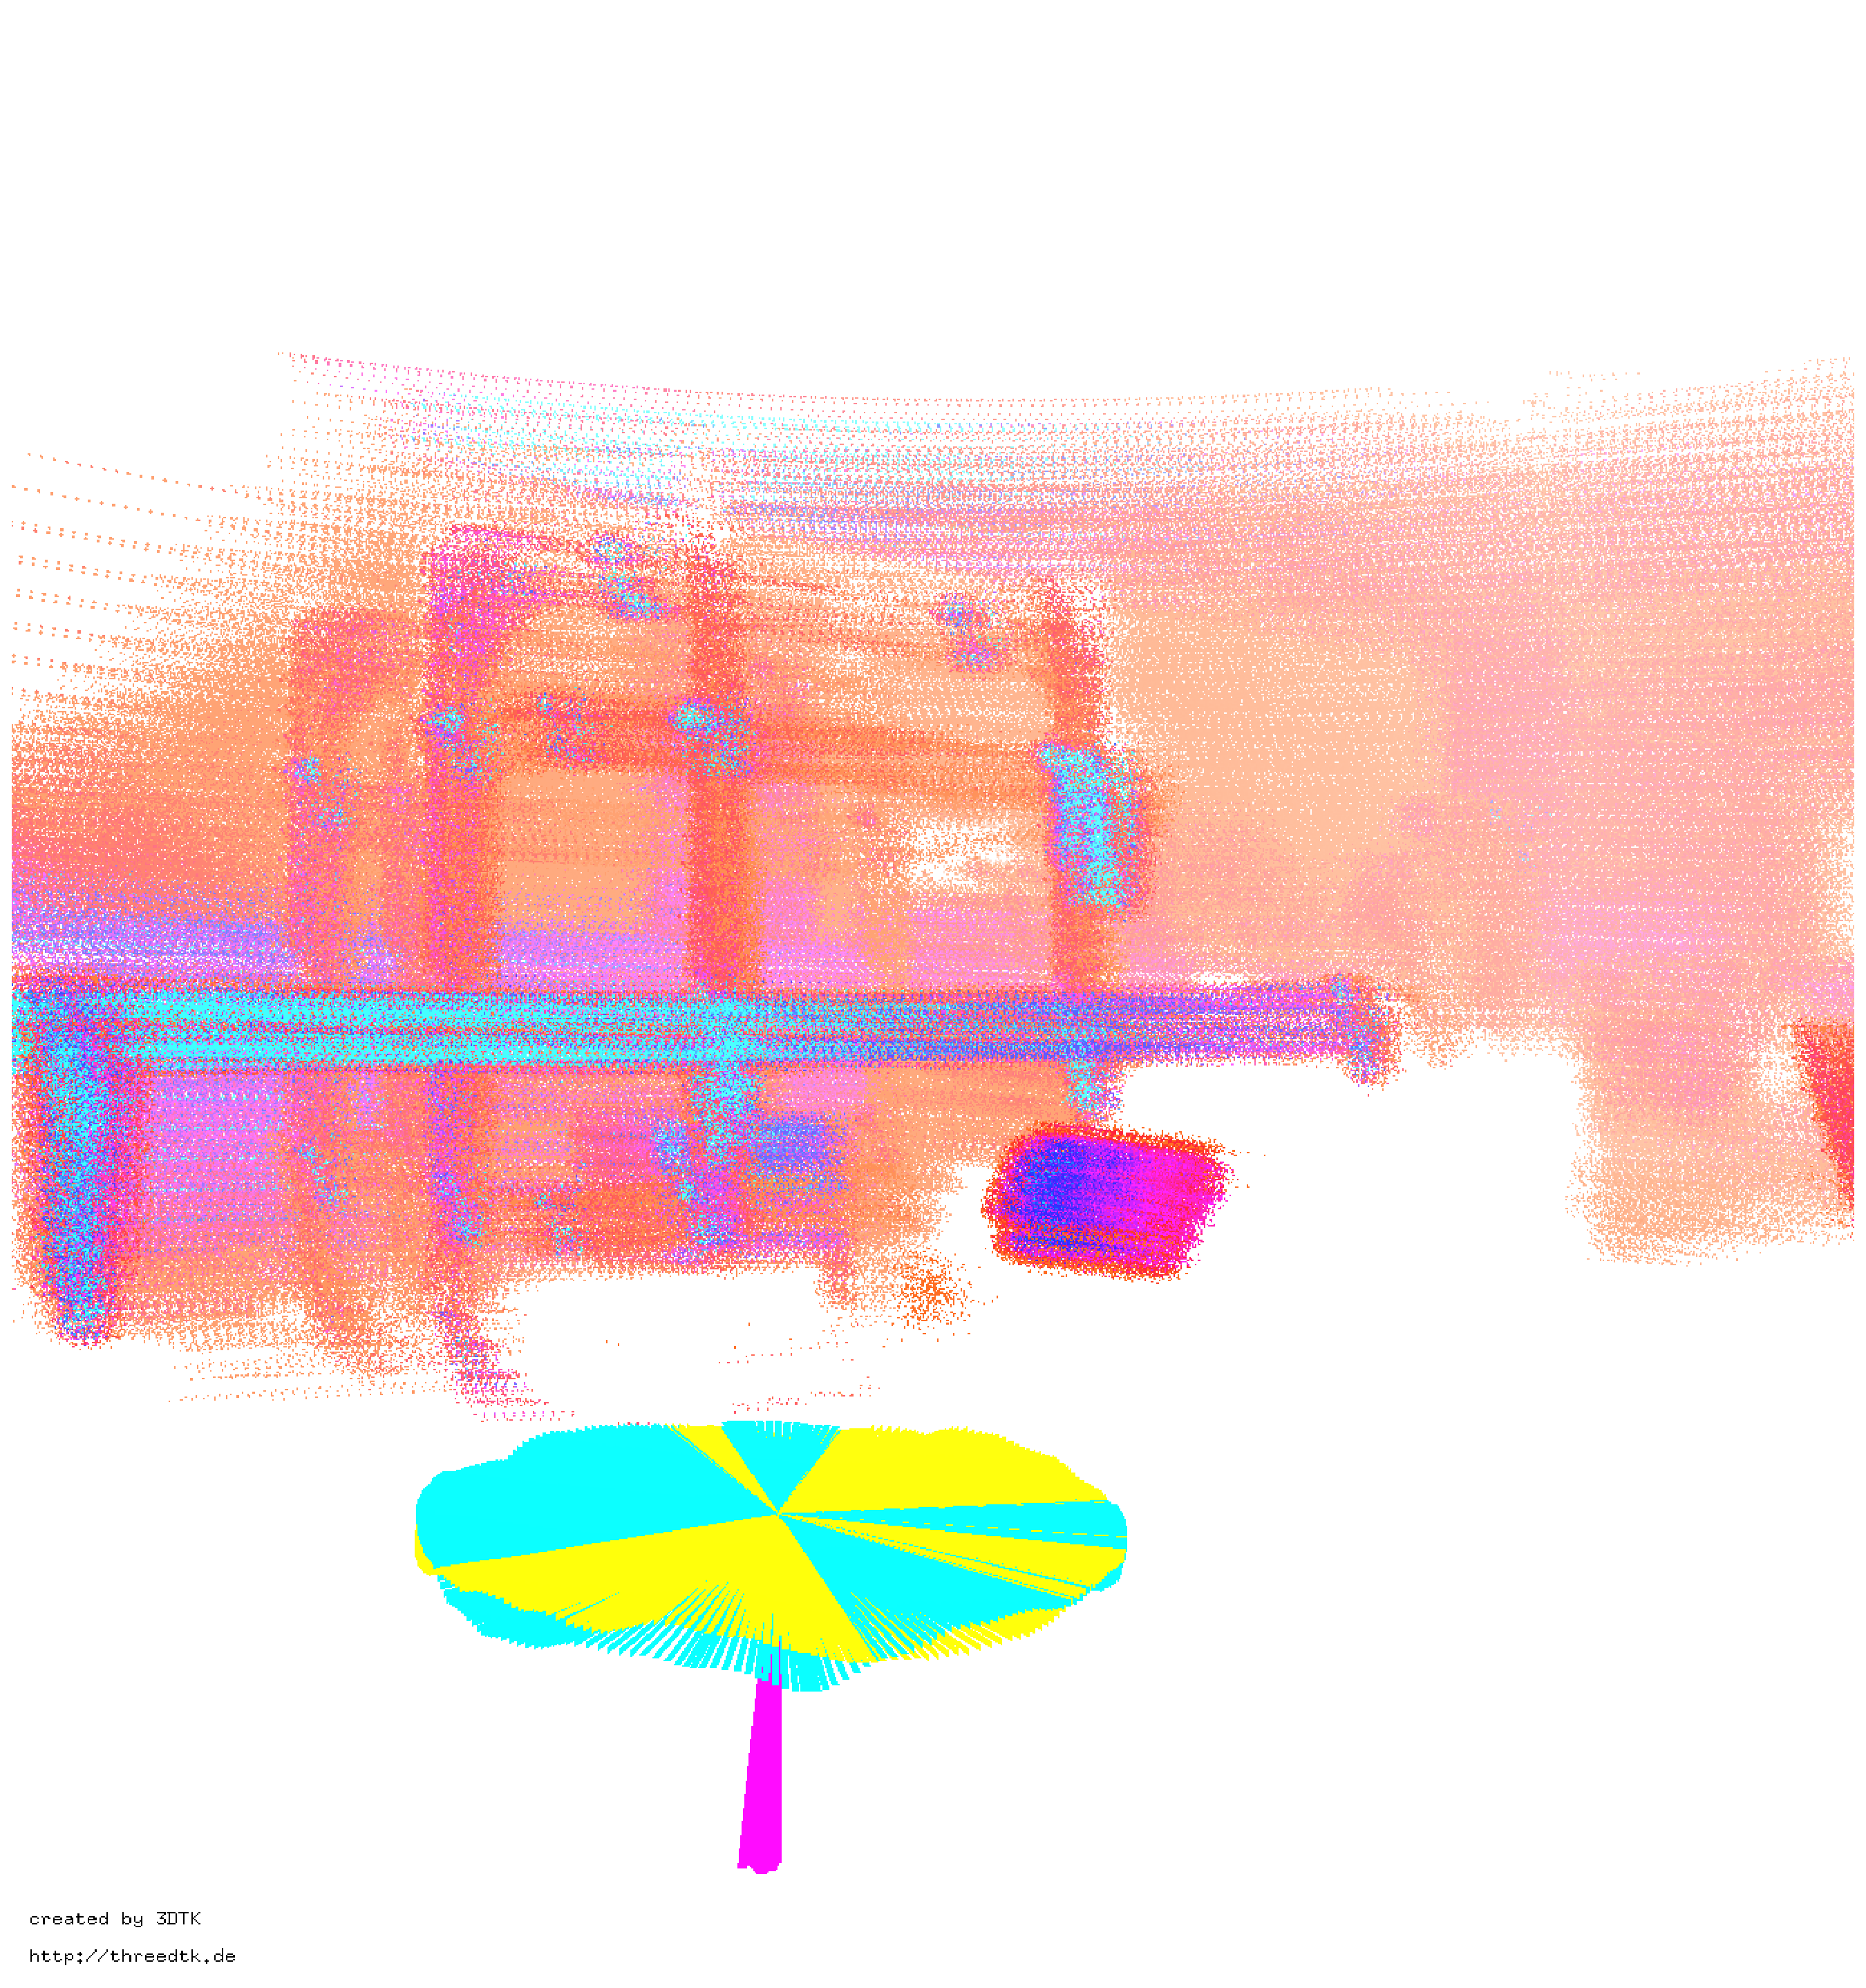
\includegraphics[width=.32\linewidth]{img/cam_yaws_before}
  \hfill
  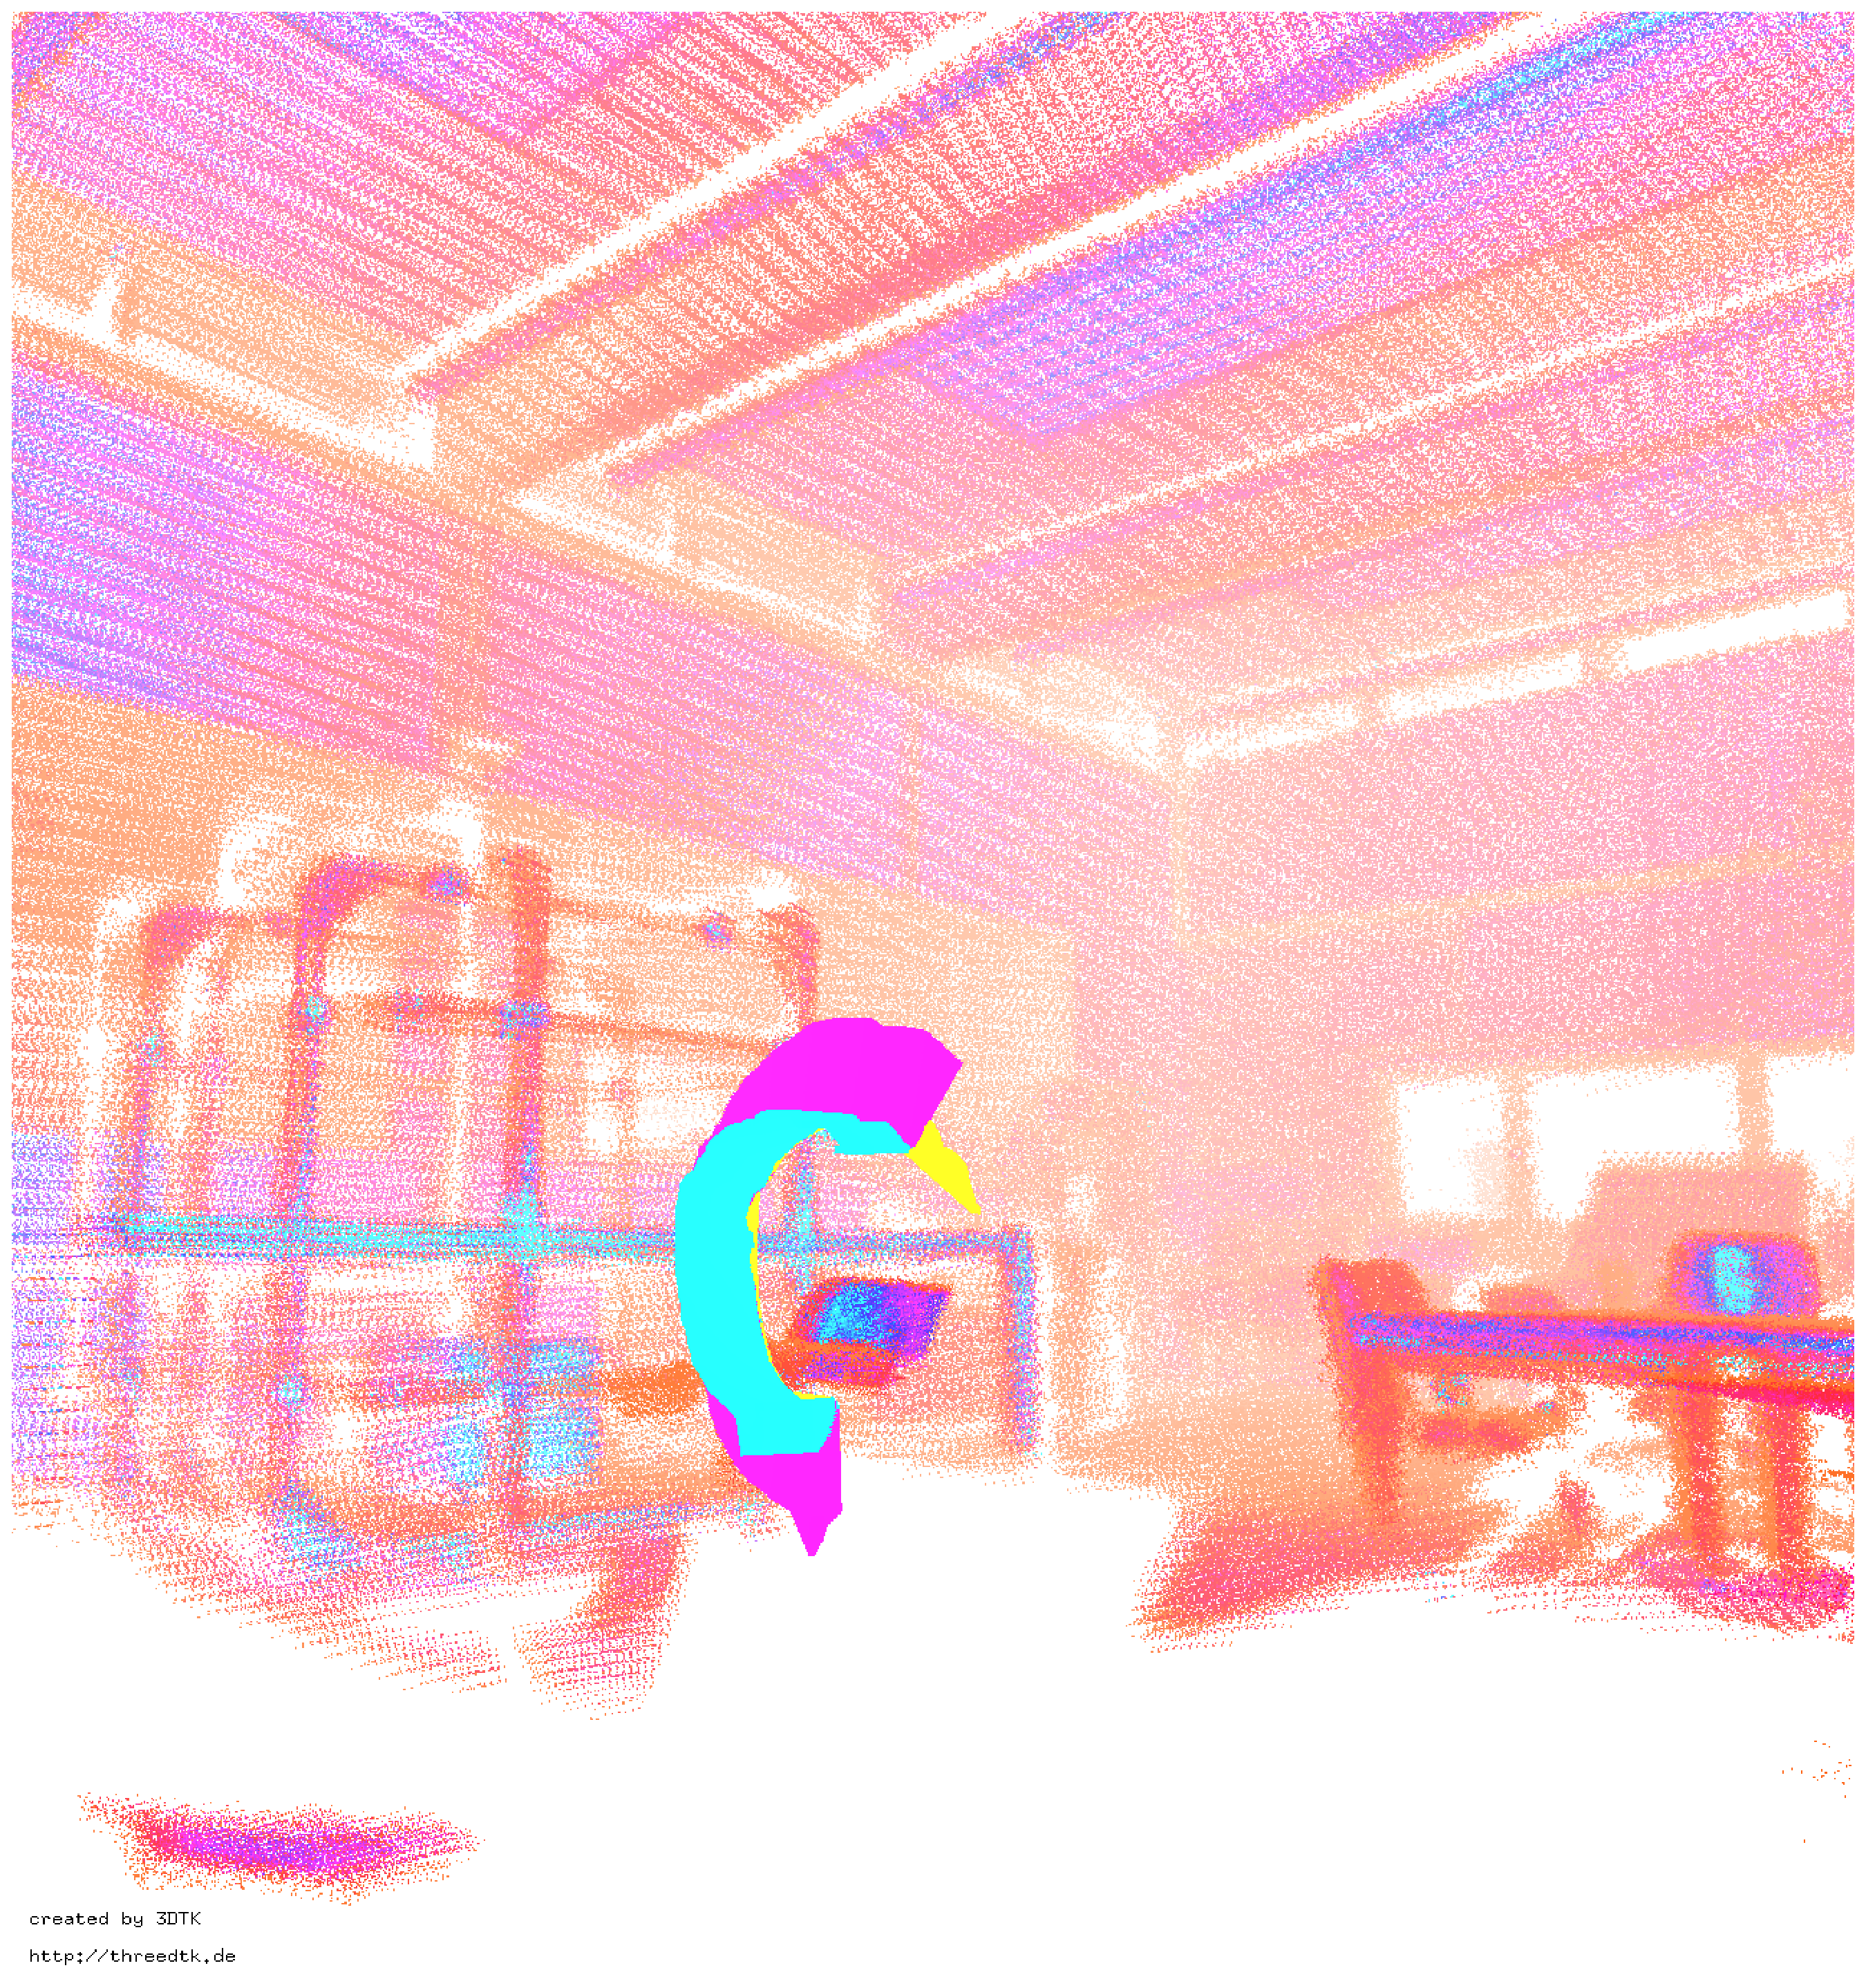
\includegraphics[width=.32\linewidth]{img/cam_rolls_aft}
  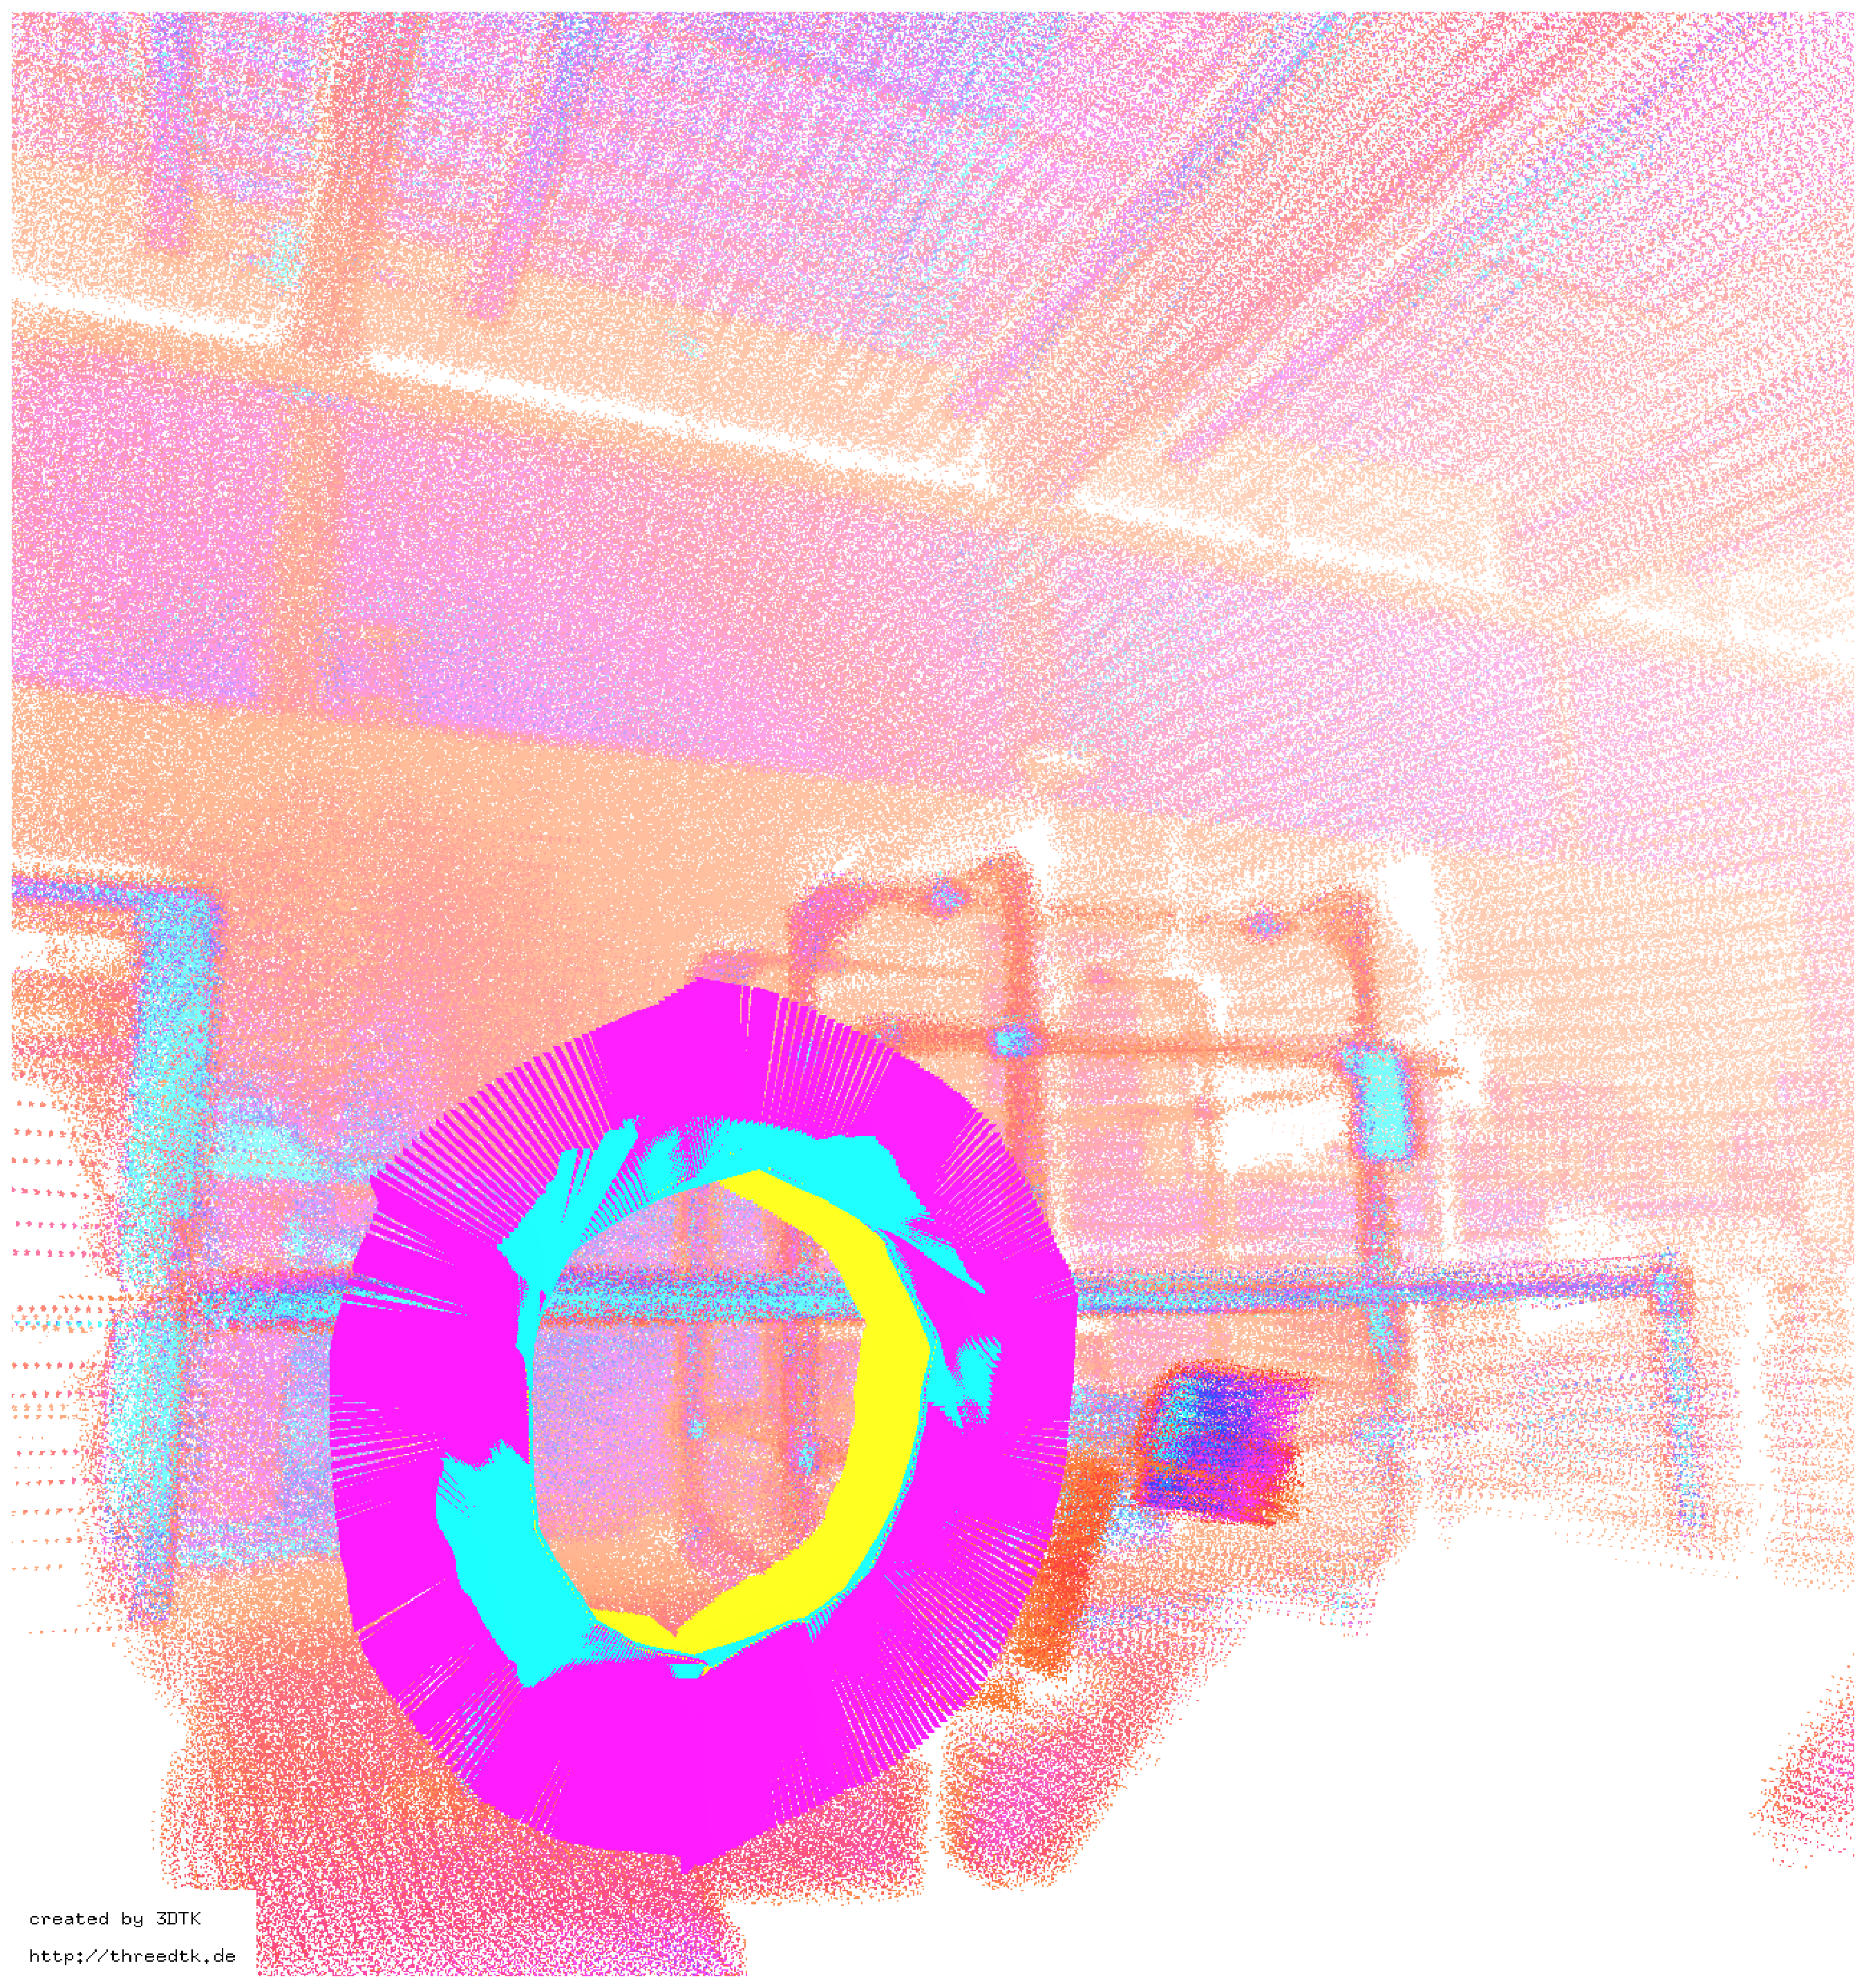
\includegraphics[width=.32\linewidth]{img/cam_pitches_aft}
  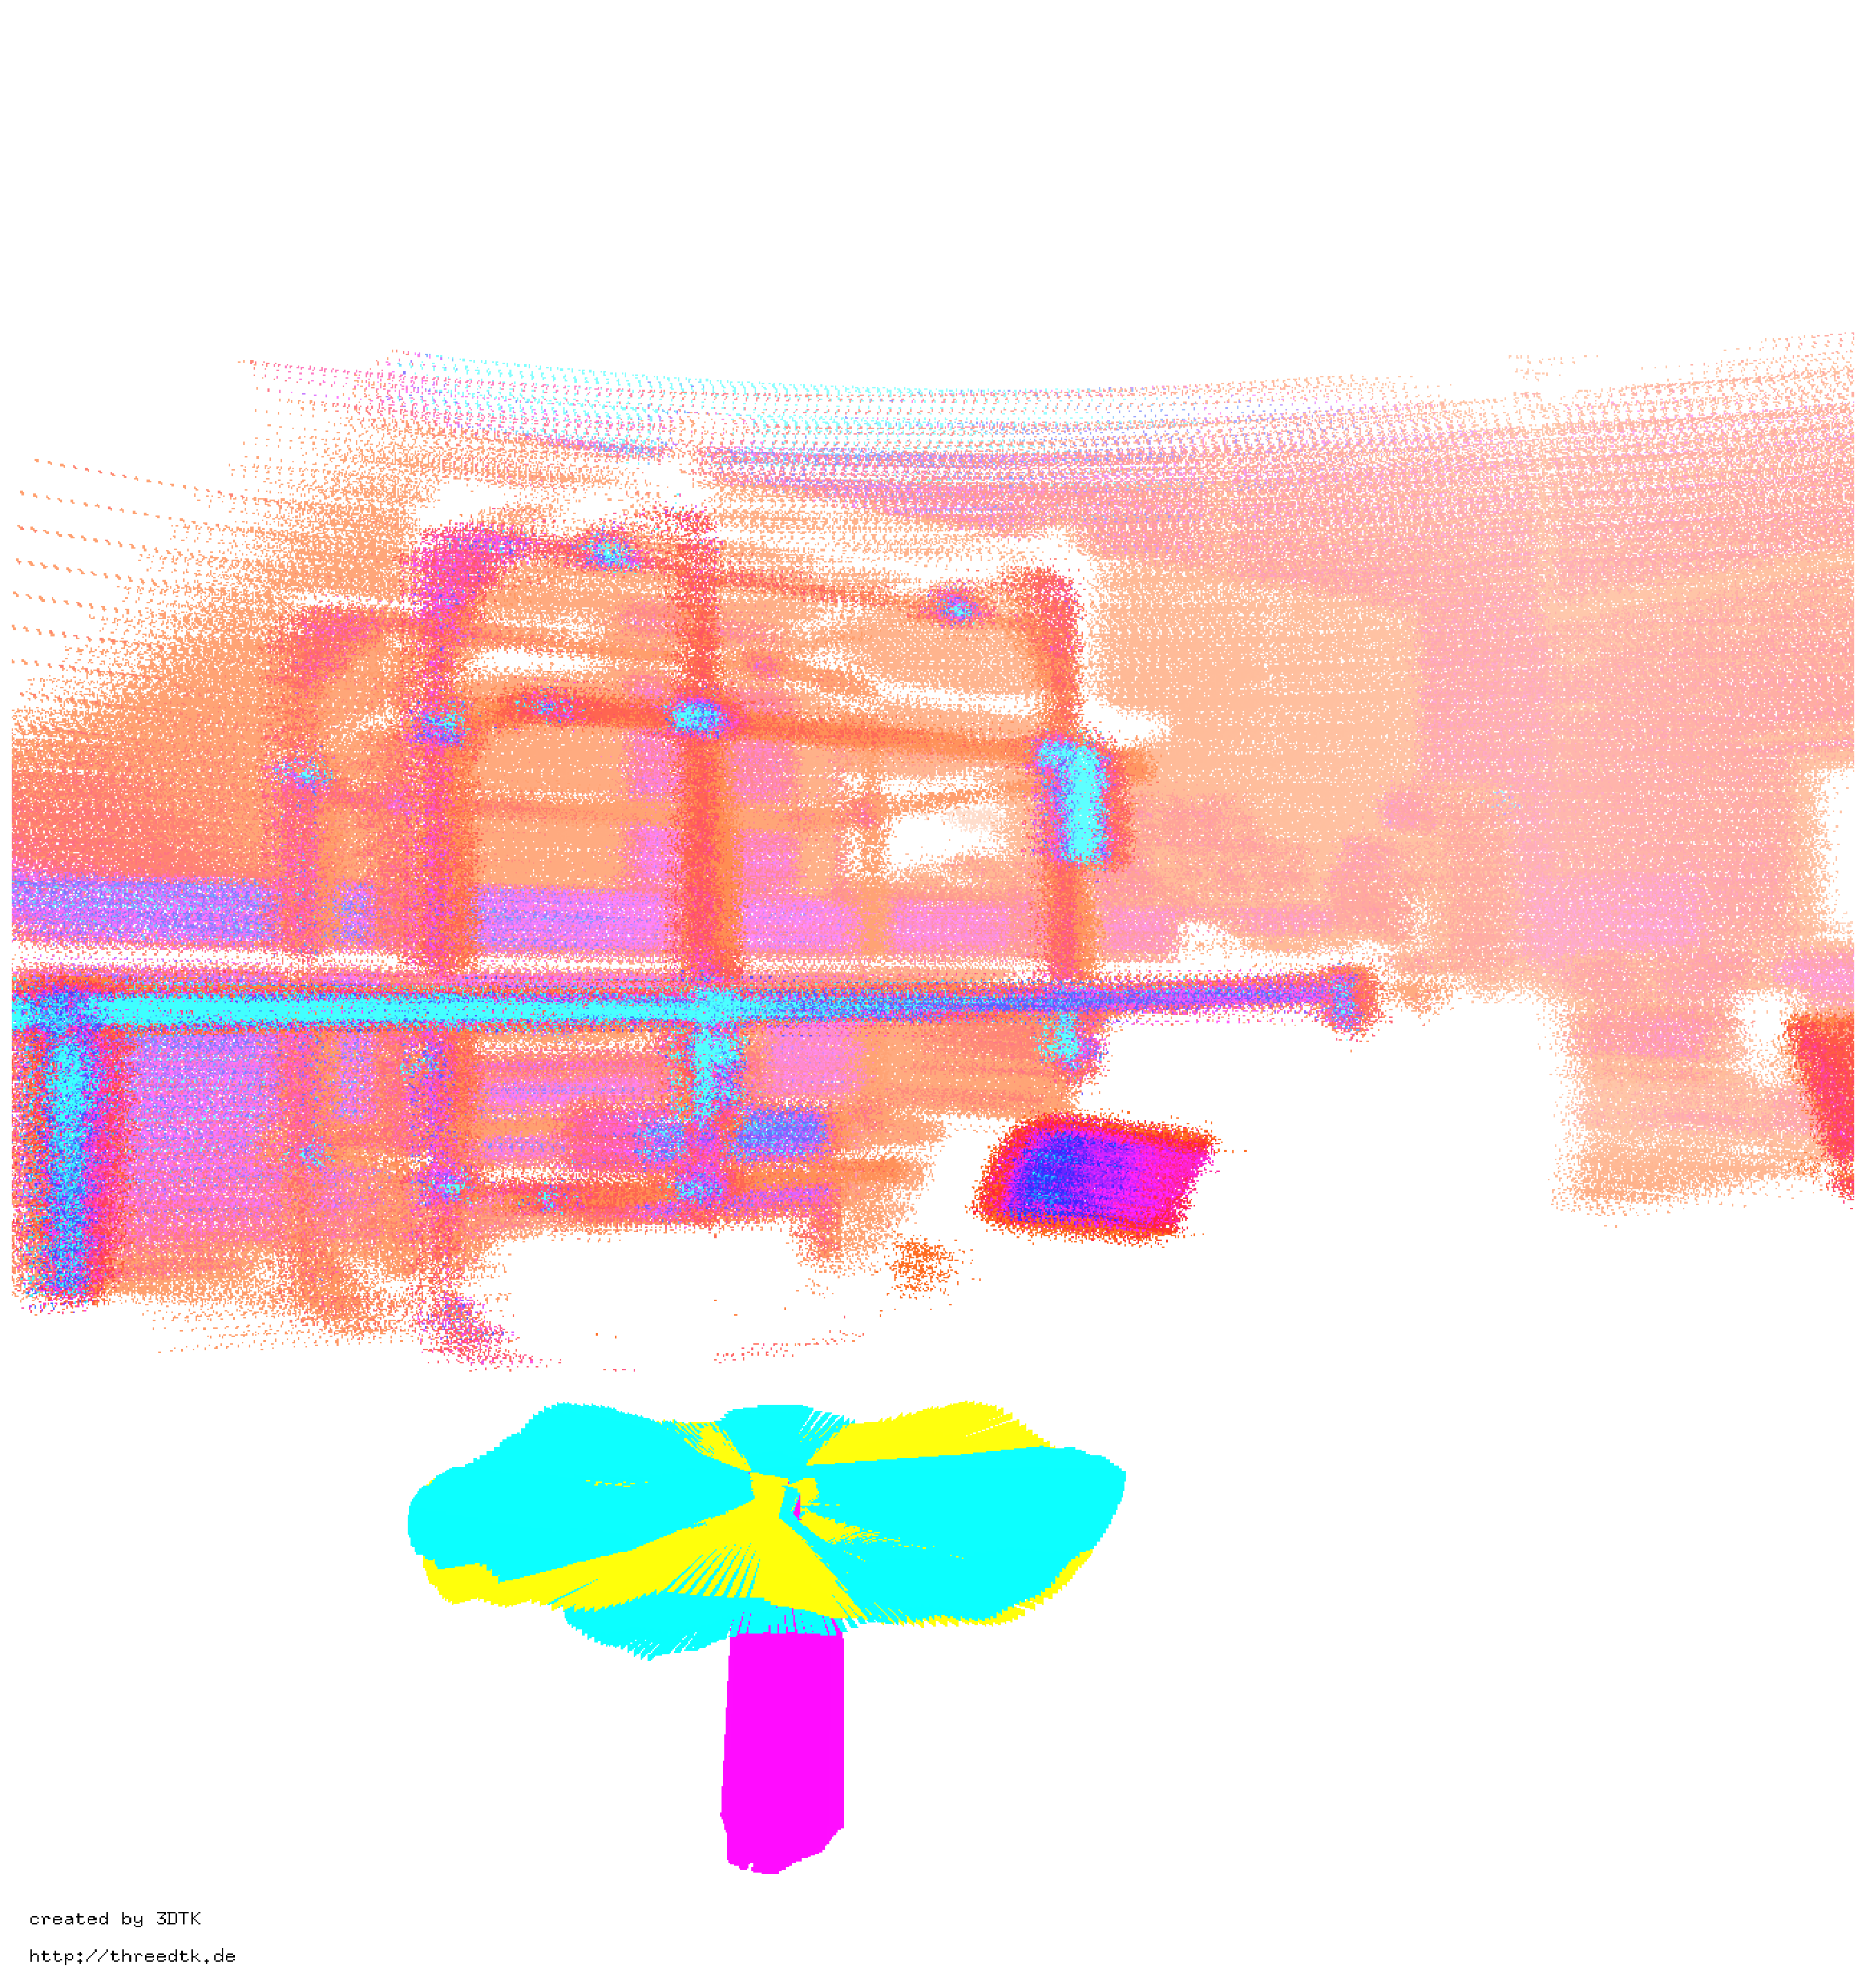
\includegraphics[width=.32\linewidth]{img/cam_yaws_aft}
  \caption{Calibration results.}
  \label{fig:circles}
\end{figure}
In this section we introduce a method of finding the extrinsic 3D translation parameters of the LiDAR sensor with respect to the center of the ball.
Knowing these offsets in all principal axes is of upmost importance for the trochoidal motion model to work.
If the ball rotates precisley around its center point, the sensor mounted rigidly inside the ball follows a circular trajectory.
The key idea behind the procedure is to measure the radii of the circular trajectory that the sensor follows when rotating around all three principal axes, then use these radii to calculate the offsets.
This is illustrated for one principal axis in Figure~\ref{fig:calibsphere}, where a rotation around the z-axis results in a radius $r_z$ which depends on the extrinsic offsets in the x and y direction, $d_x$ and $d_y$ respectivley.
The same is true for rotations around the other principal axes, leading to  
\begin{align}
  r_x^2 &= d_y^2 + d_z^2 \nonumber \\
  r_y^2 &= d_x^2 + d_z^2 \nonumber \\
  r_z^2 &= d_x^2 + d_y^2 \;,
  \label{eq:equationsystem}
\end{align}
which we solve directly by expressing the equation system in matrix-form
\begin{align}
  \begin{pmatrix}
    0 & 1 & 1 \\
    1 & 0 & 1 \\
    1 & 1 & 0
  \end{pmatrix}
  \cdot 
  \begin{pmatrix}
    d_x^2 \\
    d_y^2 \\
    d_z^2
  \end{pmatrix}
  &= 
  \begin{pmatrix}
    r_x^2 \\
    r_y^2 \\
    r_z^2
  \end{pmatrix} \nonumber \\
  \Rightarrow
  \begin{pmatrix}
    d_x^2 \\
    d_y^2 \\
    d_z^2
  \end{pmatrix}
  &= \frac{1}{2}
  \begin{pmatrix}
    -1 & \phantom{-}1 & \phantom{-}1 \\
    \phantom{-}1 & -1 & \phantom{-}1 \\
    \phantom{-}1 &  \phantom{-}1 & -1
  \end{pmatrix} 
  \cdot 
  \begin{pmatrix}
    r_x^2 \\
    r_y^2 \\
    r_z^2
  \end{pmatrix}\;.
  \label{eq:matrixform}
\end{align}
We use Equation~\eqref{eq:matrixform} to calculate the extrinsic offsets from the measured radii, as described in the next subsections.

\subsection{Estimating the radii}
In order to measure the radii as precise as possible, it is necessary to rotate the ball around its center point.
We achive this by using a 3D-printed design that houses three ball bearings, as shown in Figure~\ref{fig:calibstation}.
The ball bearings touch the spherical shell at three positions, such that any rotation of the system will happen around its center point.   
When rotating the system in that way, we first assume that the LiDAR sensor is placed in the center point and use the data of the IMUs to estimate the orientation.  
The first row of Figure~\ref{fig:circles} shows the resulting poses and misaligned point clouds, which is the input to the globally consistent, time-continuous, offline LiDAR-SLAM algorithm ``Semi-Rigid Registration''~(SRR)~\cite{srr}.
The second row of Figure~\ref{fig:circles} shows the corresponding output, i.e., the aligned point clouds and circular trajectories.
In both rows, each column corresponds to one principal axis of the system.
For the puropse of obtaining the radii, we fit circles through the SRR-estimated sensor positions for each axis using the following steps:
First, we use singular value decomposition (SVD) to fit a plane through the sensor positions, then project all sensor positions to that plane.
Second, now that the sensor positions are projected onto a 2D plane, we fit a circle by the method of least-squares to obtain the radius.
Both of these steps are common, well known techniques~\cite{geofit}.

\subsection{Obtaining the offsets}
Note that often it is not possible to direclty use the radii from the previous subsection in Equation~\eqref{eq:matrixform}.
Insisting that the offsets must not be imaginary yields the constraints
\begin{align}
  0 &< -r_x^2 + r_y^2 + r_z^2 \nonumber \\
  0 &< \phantom{-}r_x^2 - r_y^2 + r_z^2 \nonumber \\
  0 &< \phantom{-}r_x^2 + r_y^2 - r_z^2 \;,
\end{align}
which are prone to fail in the presence of measurement noise from the LiDAR or residual registration errors.
Thus, we use the sums of the squared residuals $S_i$ from the least-squares circle fitting method to calculate a $95\%$ confidence interval for the radii:
\begin{align}
  r_i \pm z_{0.975} \frac{S_i}{n-1} \frac{1}{\sqrt{n}} \;,
\end{align}
where $n$ is the number of measurments taken with the LiDAR and $z_{0.975}$ is the value of the $97.5\%$ quantile of the unit normal distribution needed for a double-sided $95\%$ confidence test.


